
\documentclass{beamer}
\usepackage[latin1]{inputenc}
%\usetheme{Montpellier}
%\usetheme{Boadilla}
%\usecolortheme[RGB={204,51,255}]{structure}
%\usecolortheme[named=purple]{structure}
\usecolortheme[RGB={62,128,62}]{structure}
%\definecolor{reddish}{rgb}{0.3,0.15,0.3}
%\definecolor{light}{rgb}{0.8,0.6,0.8}
%\definecolor{reddish}{rgb}{.5,0.15,0.15}
\definecolor{reddish}{rgb}{0.5,0.3,0.4}
%\definecolor{light}{rgb}{0.8,0.6,0.8}
\definecolor{reddish}{rgb}{.7,0.25,0.25}
\definecolor{greenish}{rgb}{.25,0.8,0.25}
\definecolor{blueish}{rgb}{.25,0.25,0.7}
\definecolor{purple}{rgb}{.5,0.0,0.5}
\usepackage{graphicx}
\usepackage{pstricks}

\newcommand{\btVFill}{\vskip0pt plus 1filll}

\setbeamertemplate{navigation symbols}{}

\newcommand{\crish}{\color{reddish}}
\newcommand{\cgish}{\color{greenish}}
\newcommand{\cbla}{\color{black}}
\newcommand{\cred}{\color{red}}
\newcommand{\cblu}{\color{blue}}
\newcommand{\cgrish}{\color{green}}

\newcommand{\sm}{\color{reddish}$}
\newcommand{\fm}{$\color{black}{}}

\newcommand{\letter}[1]{\color{blue}\texttt{#1}\color{black}}
\newcommand{\binary}[1]{\color{red}\texttt{#1}\color{black}}

\usepackage{tikz}
\usetikzlibrary{arrows,decorations.markings,positioning}
\usepackage{epstopdf}
\usetikzlibrary{fit}

\title[Information Theory lecture 7]{Differential entropy examples: information theory lecture 7}
\author{COMSM0075 Information Processing and Brain}
\institute{\texttt{comsm0075.github.io}}
\date{October 2020}

\begin{document}

\maketitle


\begin{frame}{Differential entropy}
\textbf{Differential entropy} is the name given to Shannon's entropy
for continuous probability distributions: distributions where the sample space is $\mathcal{X}\subseteq \textbf{R}^d$.


  \end{frame}


\begin{frame}{Differential entropy}
\textbf{Differential entropy} is the name given to Shannon's entropy
for continuous probability distributions.
\begin{center}
  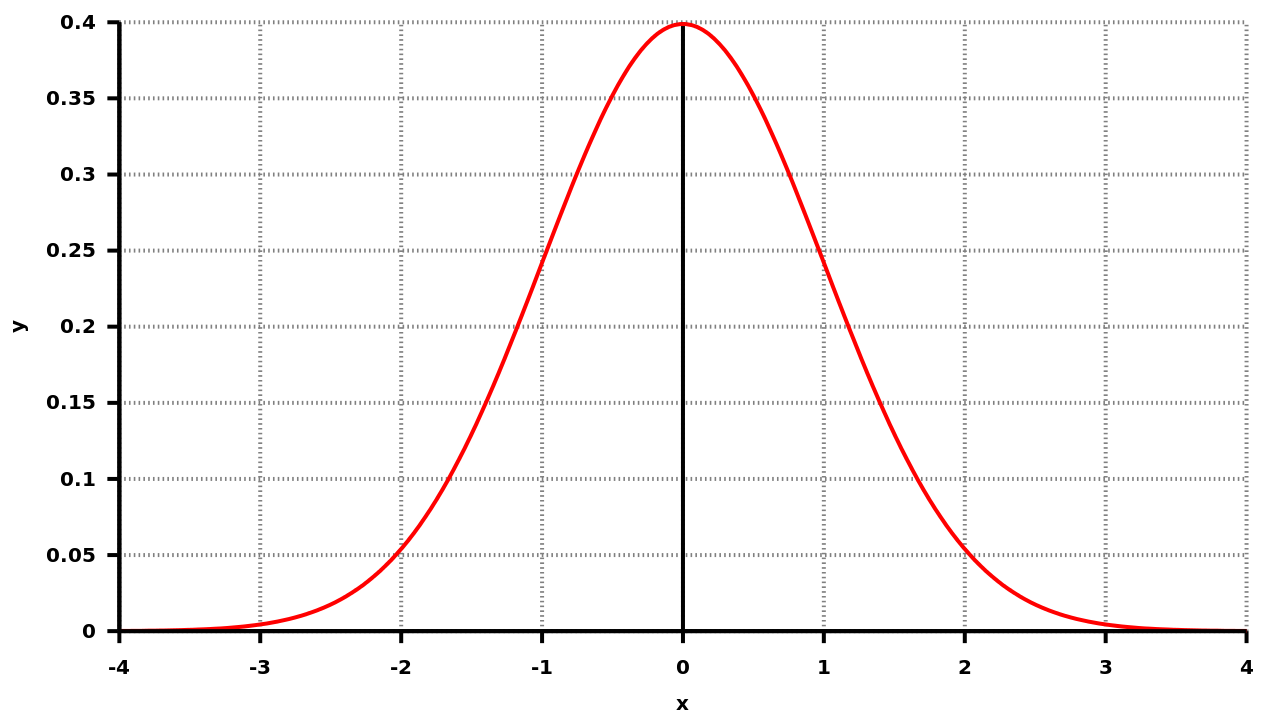
\includegraphics[width=8cm]{Gauss.svg.png}
\end{center}
\cred
$$
p(x)
$$
\cbla
\vfill
\flushright{\tiny{Image from wikipedia.}}
  \end{frame}


\begin{frame}{Differential entropy}
\textbf{Differential entropy} is the name given to Shannon's entropy
for continuous probability distributions.
\begin{center}
  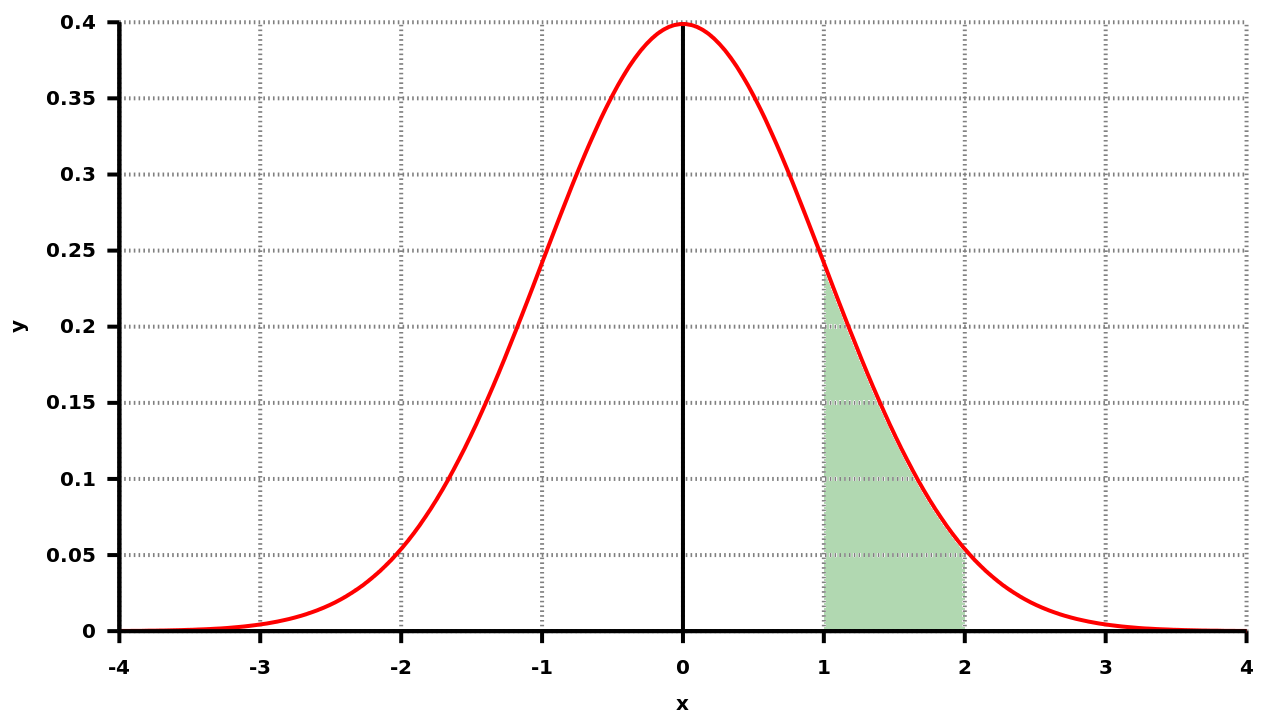
\includegraphics[width=8cm]{Gauss_area.png}
\end{center}
\cgish
  $$P(x_0\le x< x_1)=\int_{x_0}^{x_1}dx p(x)$$\cbla{} is the probability\cgish{} $x_0\le x< x_1$.
\cbla
\vfill
\flushright{\tiny{Image from wikipedia.}}
  \end{frame}



\begin{frame}{Differential entropy}
\textbf{Differential entropy} is the name given to Shannon's entropy for continuous probability distributions
\crish
$$
  h(X)=-\int dx p(x)\log_2{p(x)}
  $$ \cbla
  \end{frame}

\begin{frame}{Example - uniform}
  Consider a uniform distribution
  \crish
  $$
  p(x)=\left\{\begin{array}{ll}1/a&x\in [0,a]\\0&\mbox{otherwise}\end{array}\right.
  $$
  \cbla
  \begin{center}
    \begin{tikzpicture}
    \node[](left){$\ldots$};
    \node[right =  1cm of left](zero){};
    \node[above = 2cm of zero](overzero){};
    \node[right = 0.5cm of overzero](overa){};
    \node[below = 2cm of overa](a){};
    \node[right = 1cm of a](right){$\ldots$};
    \draw[thick] (left) -- (zero.center) -- (overzero.center) -- (overa.center) -- (a.center) -- (right);
    \draw[dotted] (zero.center) -- (a.center);
    \node[below = 0.05 cm of zero](belowzero){$0$};
    \node[below = 0.125 cm of a](belowa){$a$};
    \node[left = 0.0675 cm of overzero](leftoverzero){$1/a$};
    \end{tikzpicture}
  \end{center}
  \end{frame}


\begin{frame}{Example - uniform}
  Consider a uniform distribution
  \crish
  $$
  p(x)=\left\{\begin{array}{ll}1/a&x\in [0,a]\\0&\mbox{otherwise}\end{array}\right.
  $$
  \cbla{}so\crish{}
  $$
  h(X)=-\int_{-\infty}^{\infty}dx\, p(x)\log_2{p(x)}=-\frac{1}{a}\int_0^adx\, \log_2{\frac{1}{a}}
  $$
  \cbla{}
  and so
  \crish
  $$
  h(X)=\log_2{a}
  $$
  \cbla
  \end{frame}


\begin{frame}{Who ordered that!}

  \crish
  $$
  h(X)=\log_2{a}
  $$
  \cbla
  \begin{center}
    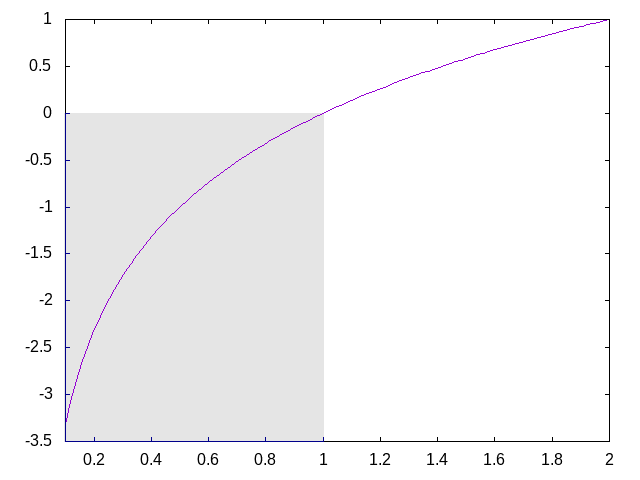
\includegraphics[width=6cm]{log_negative.png}
    \end{center}

\end{frame}

\begin{frame}{The Gau{\ss}ian distribution}
\crish
$$
p(x)=\frac{1}{\sqrt{2\pi \sigma^2}}\exp\left(\frac{-x^2}{2\sigma^2}\right)
$$
\cbla
Substitute and integrate by parts to get
\crish
$$
  h(X)=\frac{1}{2}\log_2{2\pi e \sigma^2}
  $$
\cbla
where the \crish$e$\cbla{} is just the exponential \crish$\exp{(1)}$\cbla.
\end{frame}

\begin{frame}{More of the negative values}
\begin{quote}
As with the uniform
distribution, this formula can give a positive or negative number
depending on the size of \crish$\sigma$\cbla. Interestingly it can be proved that
for fixed variance the Gau{\ss}ian has the highest entropy.
\end{quote}
\end{frame}


\begin{frame}{Densities are not probabilities}
  \cred
  discrete case $p(x)$ is the probability of $X=x$\\
  \cgish
  \vskip 1cm
  continuous case
  $$\int_{x_0}^{x_1}dx p(x)$$ is the probability $x_0\le x< x_1$.
\end{frame}


\begin{frame}{Densities are not probabilities}
The usual sums and probabilities go to integrals and densities doesn't work because there is a \cblu$p$\cbla{} in the log:
\crish
$$
  h(X)=-\int dx p(x)\log_2{\cblu{}p(x)\crish}
  $$ \cbla
  \end{frame}
  

\begin{frame}{Real numbers are like an infinity of numbers}
  \crish

  1.618033988749894848204586834365638117720309179805762862135
  44862270526046281890244970720720418939113748475408807538689
  17521266338622235369317931800607667263544333890865959395829
  05638322661319928290267880675208766892501711696207032221043
  21626954862629631361443814975870122034080588795445474924618
  56953648644492410443207713449470495658467885098743394422125
  44877066478091588460749988712400765217057517978834166256249
  40758906970400028121042762177111777805315317141011704666599
  14669798731761356006708748071013179523689427521948435305678
  30022878569978297783478458782289110976250030269615617002504
  64338243776486102838312683303724292675263116533924731671112
  11588186385133162038400522216579128667529465490681131715993
  43235973494985090409476213222981017261070596116456299098162
  90555208524790352406020172799747175342777592778625619432082
  7505131218156285512224809394$\ldots$

\end{frame}


\begin{frame}{We can't really see all the numbers}
  \crish
  1.61\color{lightgray}8033988749894848204586834365638117720309179805762862135
  44862270526046281890244970720720418939113748475408807538689
  17521266338622235369317931800607667263544333890865959395829
  05638322661319928290267880675208766892501711696207032221043
  21626954862629631361443814975870122034080588795445474924618
  56953648644492410443207713449470495658467885098743394422125
  44877066478091588460749988712400765217057517978834166256249
  40758906970400028121042762177111777805315317141011704666599
  14669798731761356006708748071013179523689427521948435305678
  30022878569978297783478458782289110976250030269615617002504
  64338243776486102838312683303724292675263116533924731671112
  11588186385133162038400522216579128667529465490681131715993
  43235973494985090409476213222981017261070596116456299098162
  90555208524790352406020172799747175342777592778625619432082
  7505131218156285512224809394$\ldots$
\cbla
  \end{frame}


\begin{frame}{Sensitivity}
 We need to model the sensitivity of the receiver as well the
 behaviour of the source.
  \begin{center}

\includegraphics[width=7cm]{cont1.png}
  \end{center}  
\end{frame}


\begin{frame}{Sensitivity}
 We need to model the sensitivity of the receiver as well the
 behaviour of the source.
  \begin{center}
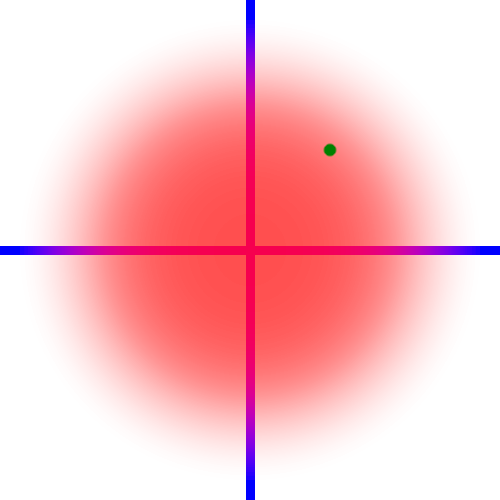
\includegraphics[width=7cm]{cont2.png}
  \end{center}  
\end{frame}


\begin{frame}{Sensitivity}
 We need to model the sensitivity of the receiver as well the
 behaviour of the source.
  \begin{center}
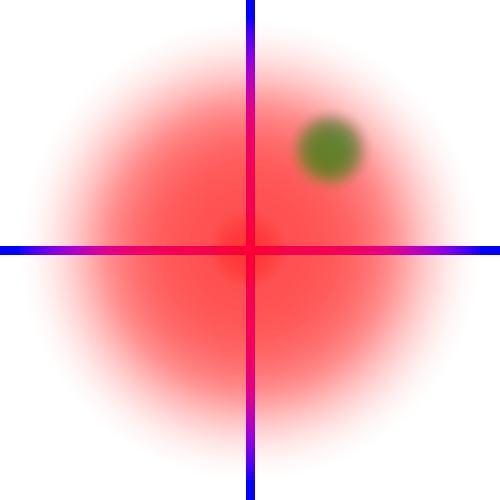
\includegraphics[width=7cm]{cont3.png}
  \end{center}  
\end{frame}


\begin{frame}{Sensitivity}
 We need to model the sensitivity of the receiver as well the
 behaviour of the source.
  \begin{center}
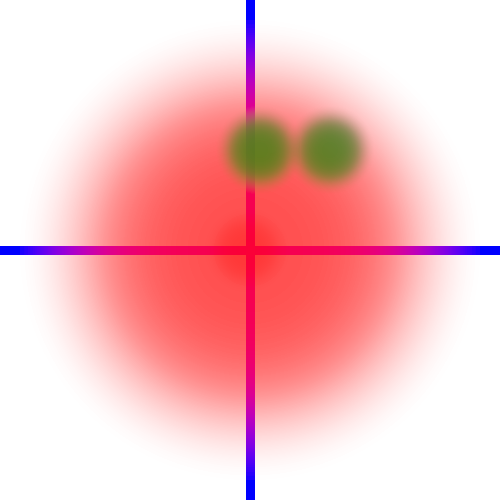
\includegraphics[width=7cm]{cont4.png}
  \end{center}  
\end{frame}


\begin{frame}{Sensitivity}
Maybe \crish$I(X,Y)$\cbla{} is what we really want.
\end{frame}



\end{document}

